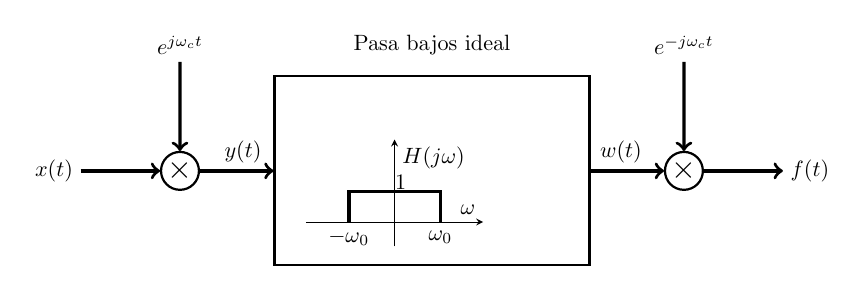
\begin{tikzpicture}[scale=0.8, transform shape]
    \node[rectangle, draw, thick, minimum height=3cm, minimum width=5cm] (hpb) at (0,0) {} ;
    \begin{axis}[
        x=0.04\textwidth,y=0.04\textwidth,
        axis y line=center,
        axis x line=middle,
        xlabel=$\omega$,ylabel={ $H(j\omega)$},
        xmin=-2.9,xmax=2.9,
        ymin=-0.8,ymax=2.7,
        ticks=none,
        at={(-2cm,-1.2cm)}
        ]
        \addplot[
        black,
        ultra thick
        ] coordinates {
            (-1.5,0) (-1.5,1) (1.5,1) (1.5,0)
        } ;
        \node at (-1.5,-.5) {$-\omega_0$};
        \node at (1.5,-.5) {$\omega_0$};
        \node at (0.2,1.3) {1} ;
    \end{axis} 
    \node[yshift=2cm] (hpb_label) at (hpb) {Pasa bajos ideal} ;

    \node[circle,draw,thick,inner sep=0.03cm, xshift=4cm] (mult_after) at (hpb) {\Large $\times$} ;
    \node[circle,draw,thick,inner sep=0.03cm, xshift=-4cm] (mult_before) at (hpb) {\Large $\times$} ;
    \node[yshift=2cm] (exp_after) at (mult_after) {$e^{-j\omega_c t}$} ;
    \node[yshift=2cm] (exp_before) at (mult_before) {$e^{j\omega_c t}$} ;
    \node[xshift=-2cm] (x_t) at (mult_before) {$x(t)$} ;
    \node[xshift=1cm,yshift=0.3cm] (y_t) at (mult_before) {$y(t)$} ;
    \node[xshift=2cm] (f_t) at (mult_after) {$f(t)$} ;
    \node[xshift=-1cm,yshift=0.3cm] (w_t) at (mult_after) {$w(t)$} ;

    \draw[->, very thick] (x_t.east) -- (mult_before.west) ;
    \draw[->, very thick] (mult_before.east) -- (hpb.west) ;
    \draw[->, very thick] (hpb.east) -- (mult_after.west) ;
    \draw[->, very thick] (mult_after.east) -- (f_t.west) ;
    \draw[->, very thick] (exp_before.south) -- (mult_before.north);
    \draw[->, very thick] (exp_after.south) -- (mult_after.north);
\end{tikzpicture}